%\documentclass[class=report , crop=false, multi={itemize, figure}, float=false]{standalone}%Experimental
\documentclass[class=book , crop=false]{standalone}

\usepackage{import} % Required for importing other .tex docs.  (import uses everything bw Begin and End Doc)
\usepackage{float} % Required for specifying the exact location of a figure or table
\usepackage{graphicx} % Required for including images
\usepackage{wrapfig}
\usepackage[pdftex,breaklinks,colorlinks=true,linkcolor=black,citecolor=blue,urlcolor=red,linktocpage=false,pagebackref=true,filecolor=magenta]{hyperref}%http://www.tug.org/applications/hyperref/manual.html#x1-100003.6
\usepackage{cite}
\usepackage[toc,title,page]{appendix}
\usepackage{pdfpages} % enables loading a pdf into the doc
\usepackage{makeidx}
\usepackage{glossaries} % must be after hyperref
\usepackage{blindtext}
\usepackage{enumitem}
%\usepackage{caption}

%\setlist[description]{leftmargin=\parindent,labelindent=\parindent}

%\renewcommand*{\bibname}{References} % renames the bibliography

\newcommand{\HRule}{\rule{\linewidth}{0.5mm}} % Command to make the lines in the title page

\graphicspath{{img/}{GIS_ChampionSection/img/}{awardsChapter/GIS_ChampionSection/img/}{brandPart/awardsChapter/GIS_ChampionSection/img/}{img/}{pairedProgSection/img/}{methodChapter/pairedProgSection/img/}{methodPart/methodChapter/pairedProgSection/img/}{documentationSection/img/}{methodChapter/documentationSection/img/}{methodPart/methodChapter/documentationSection/img/}{docStorageOrgSection/img/}{methodChapter/docStorageOrgSection/img/}{methodPart/methodChapter/docStorageOrgSection/img/}{QGisSection/img/}{toolsChapter/QGisSection/img/}{servicePart/toolsChapter/QGisSection/img/}{ESRISection/img/}{toolChapter/ESRISection/img/}{servicePart/toolChapter/ESRISection/img/}{../../../../source/}{../../source/}{servicePart/applicationsChapter/treasurerSection/img/}}

%\setlength\parindent{0pt} % eliminates indents


\def\titlename{Parcel Editing with COGO Tools in QGIS}

\title{\HRule % Horizontal Line added
\\[.4cm] % space
\begin{figure}[H] % included image
\begin{center}	% centered horizontally
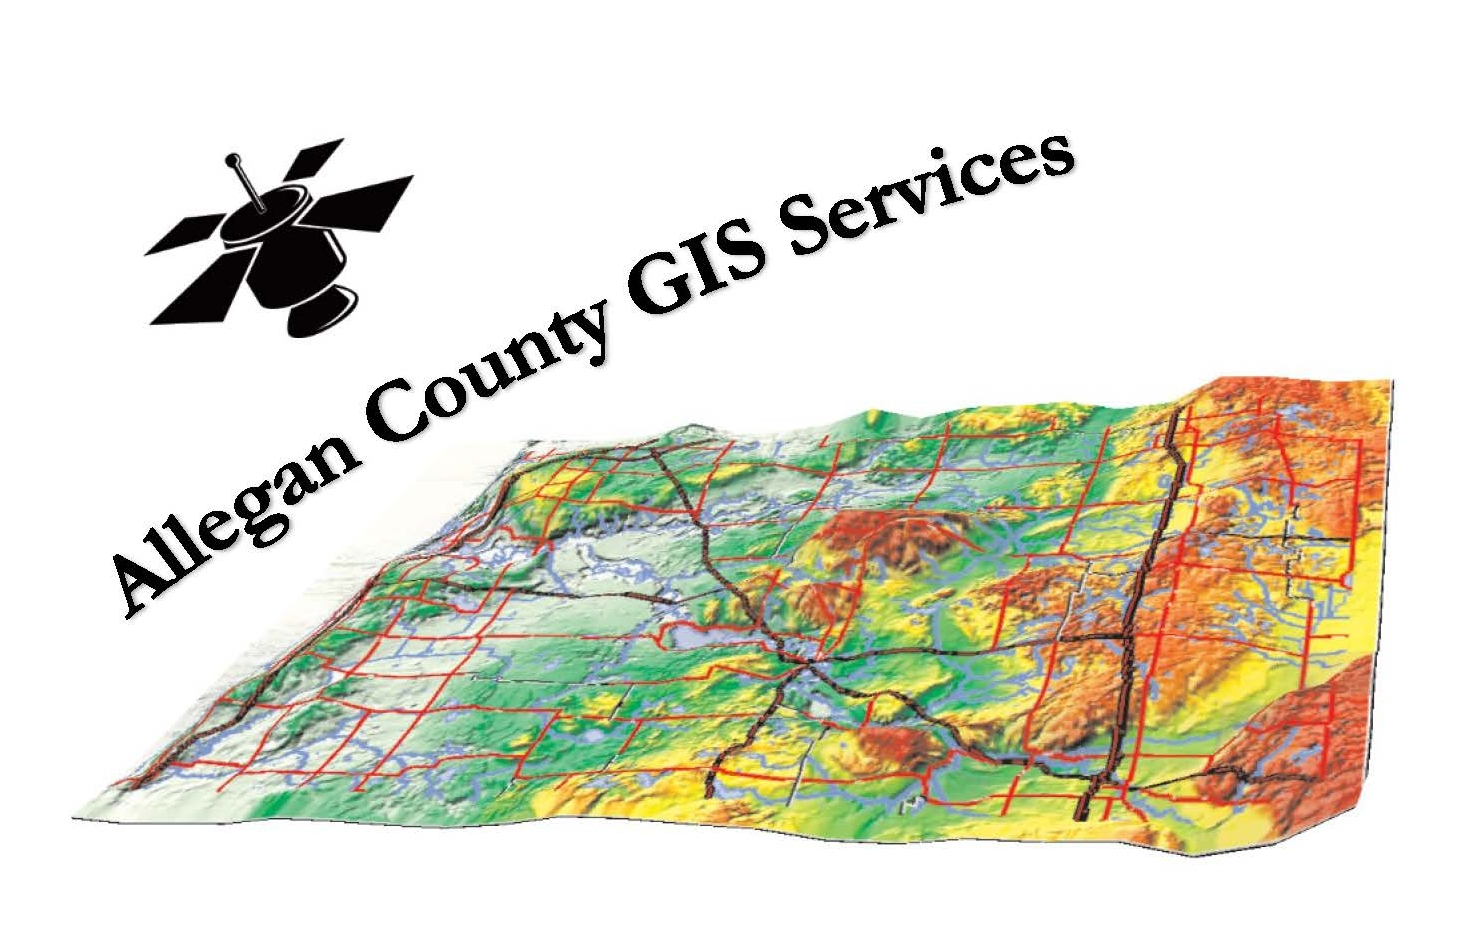
\includegraphics[scale=.45]{GIS_Logo_better.jpg}
\end{center}
\end{figure}
\Huge \bfseries \titlename \\ % Title text
\HRule \\[.4cm] % Horizontal Line added
\author{\Large Allegan County GIS \\\Large www.allegancounty.org/gis} % defines author
}  % closing brace for title

\begin{document}% Document Begins

\ifstandalone
%\frontmatter % turns off chapter numbering and uses roman numerals for page numbers
\maketitle % creates title page and blank page after title page
\tableofcontents % creates TOC and blank page
\clearpage
%\mainmatter % turns on chapter numbering, resets page numbering and uses arabic numerals for page numbers
\fi

\subsection{Using COGO Tools in QGIS}
\medskip 
\subsubsection{\Large Set up the Azimuth and Distance Plugin \\\small(Azd Plugin).}
%\subparagraph{After starting QGIS in the basemap}
\medskip
\large In the Plugins drop down(1), \large under the topography group\\\Large select the \textbf {Azd Plugin(2)}(see fig.).
\begin{figure}[H] % included image
\begin{center}
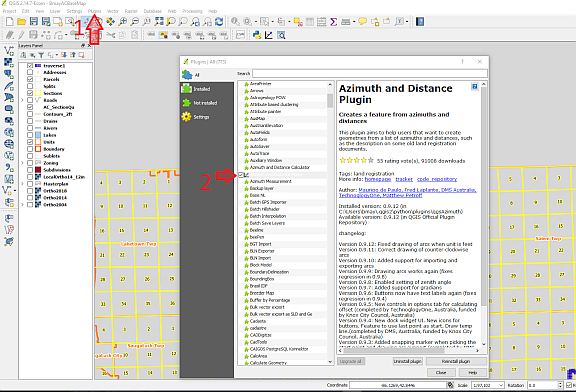
\includegraphics[scale=.30]{1.png}
\end{center}
\caption{launch plugin}
\end{figure}
\clearpage
		
\large Note here which layer is active (see fig.).
\begin{figure}[H] % included image
\begin{center}
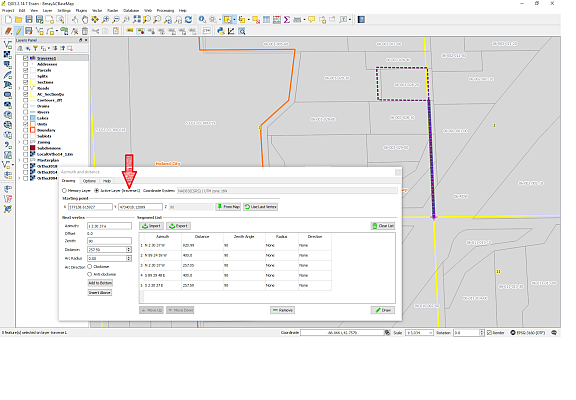
\includegraphics[scale=.26]{2.png}
\end{center}
\caption{check active layer}
\end{figure}

%\clearpage

If necessary, left click the layer \textbf {\emph{traverse 1}} in Layer Panel to activate it(see fig.).
\begin{figure}[H] % Example of including images
\begin{center}
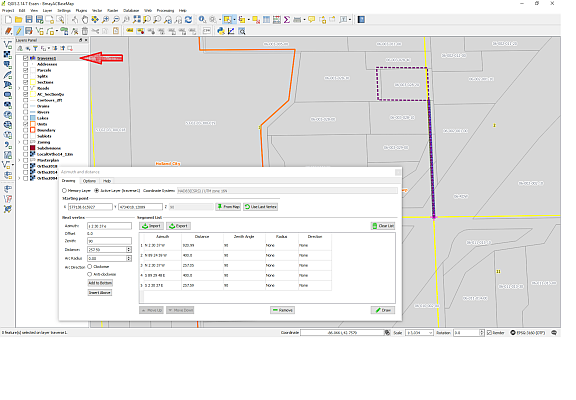
\includegraphics[scale=.2]{3.png}
\end{center}
\caption{activate layer}
\end{figure}

\clearpage

\paragraph{Configure Options}
\large On Options Tab: Select Boundary, Bearing, Feet, and Degree radio buttons.
\begin{figure}[H]
\begin{center}
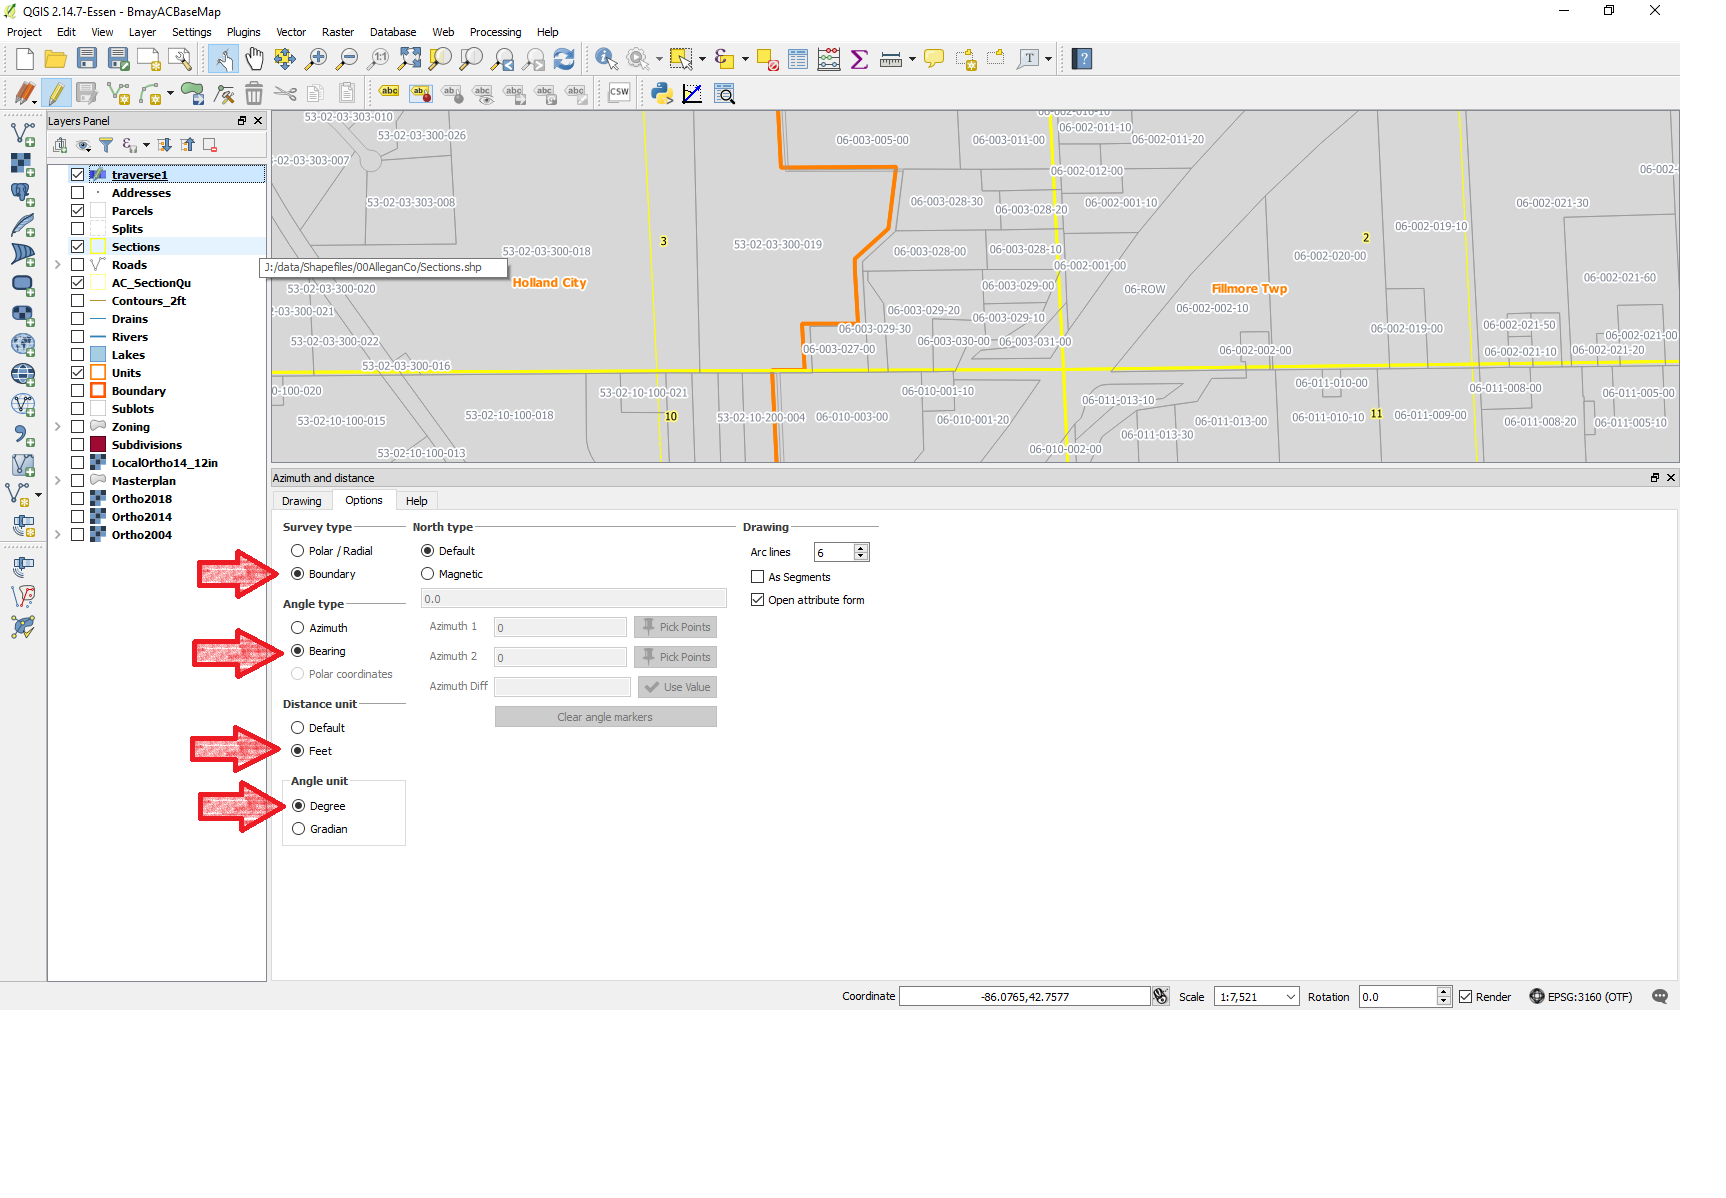
\includegraphics[scale=.25]{4.png}
\end{center}
\caption{Plugin Options}
\end{figure}
\clearpage

\paragraph{Using the tool}
\large Boundary descriptions are entered into the Drawing Tab. Azimuth (bearing) and Distance are the important boxes (Set Offset = 0 and Zenith = 90 and ignore)(see below).
\begin{figure}[H]
\begin{center}
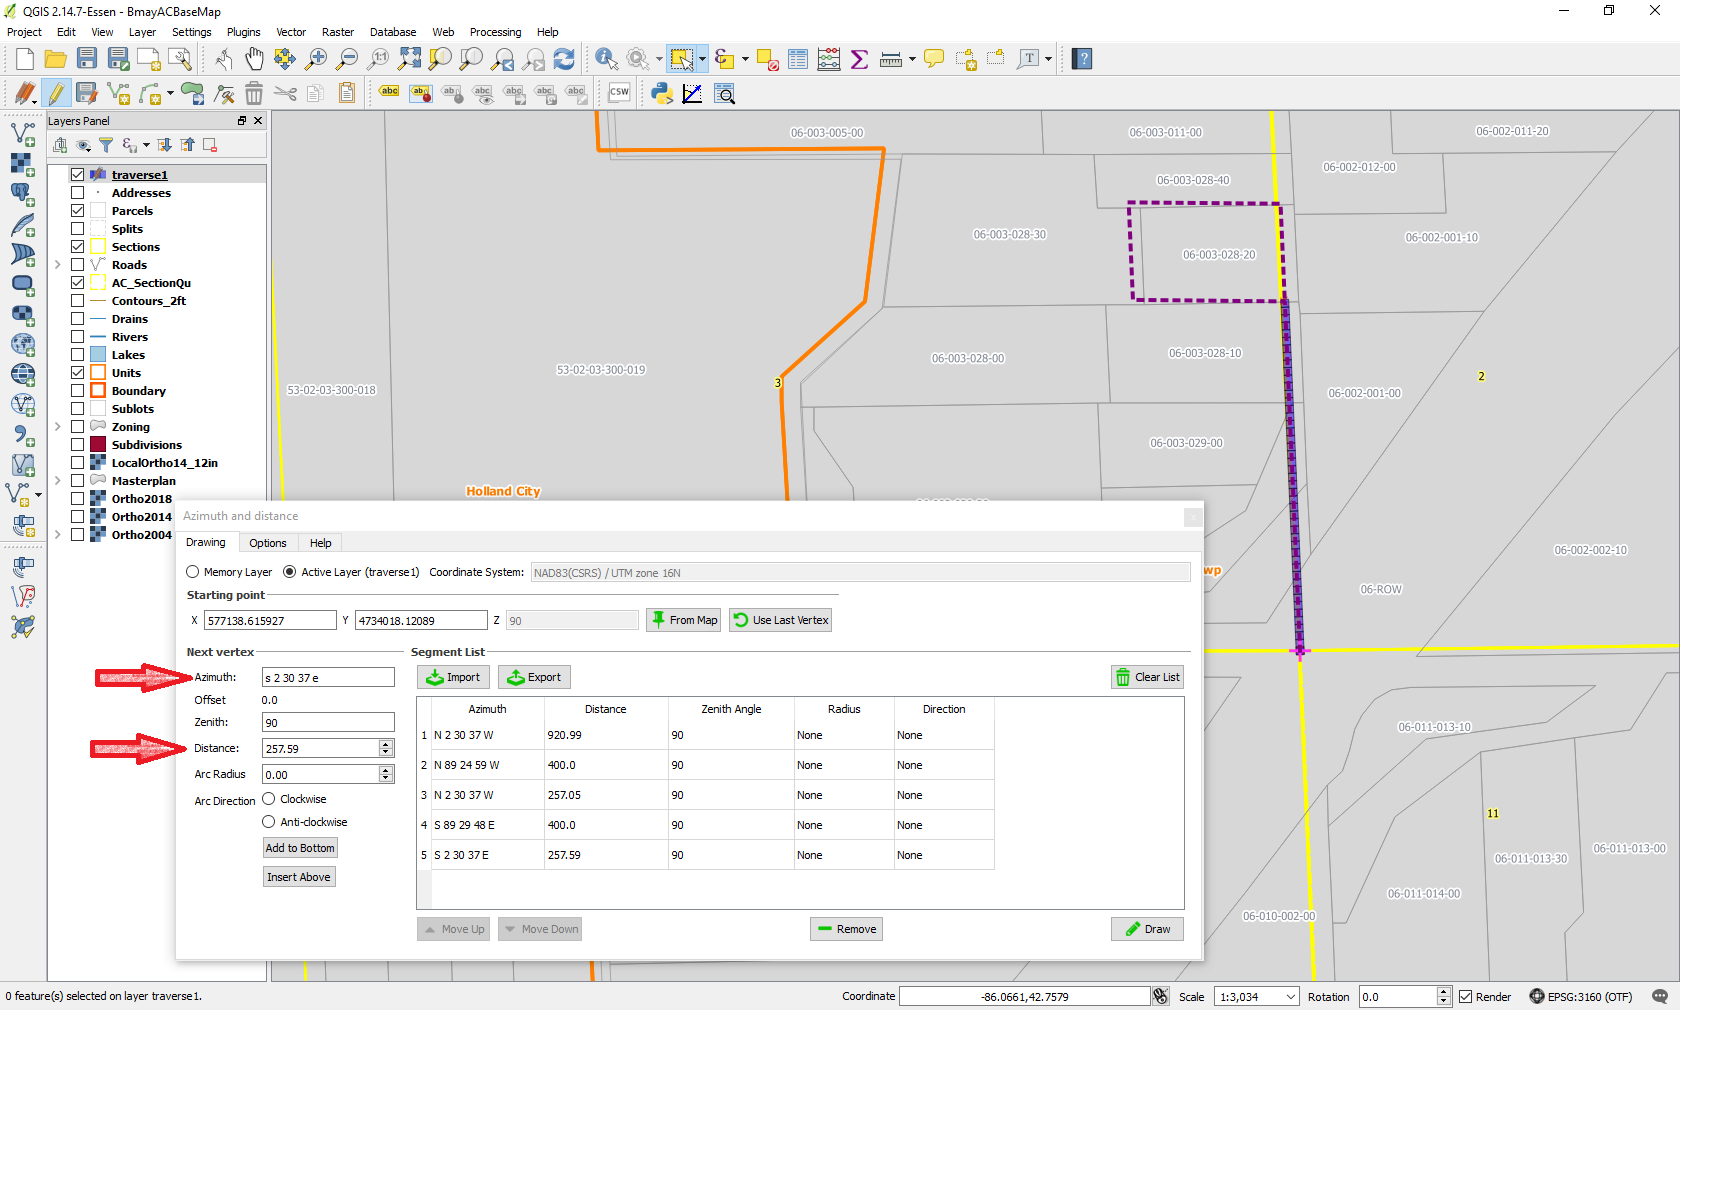
\includegraphics[scale=.25]{5.png}
\end{center}
\caption{Entering Bounds}
\end{figure}

\clearpage

\subsubsection{Configure editing environment}
\Large Use Settings Dropdown and Snapping Options to enable snapping to Sections, Quarter Sections, and or Parcels if desired (see fig.).

\begin{figure}[H]
\begin{center}
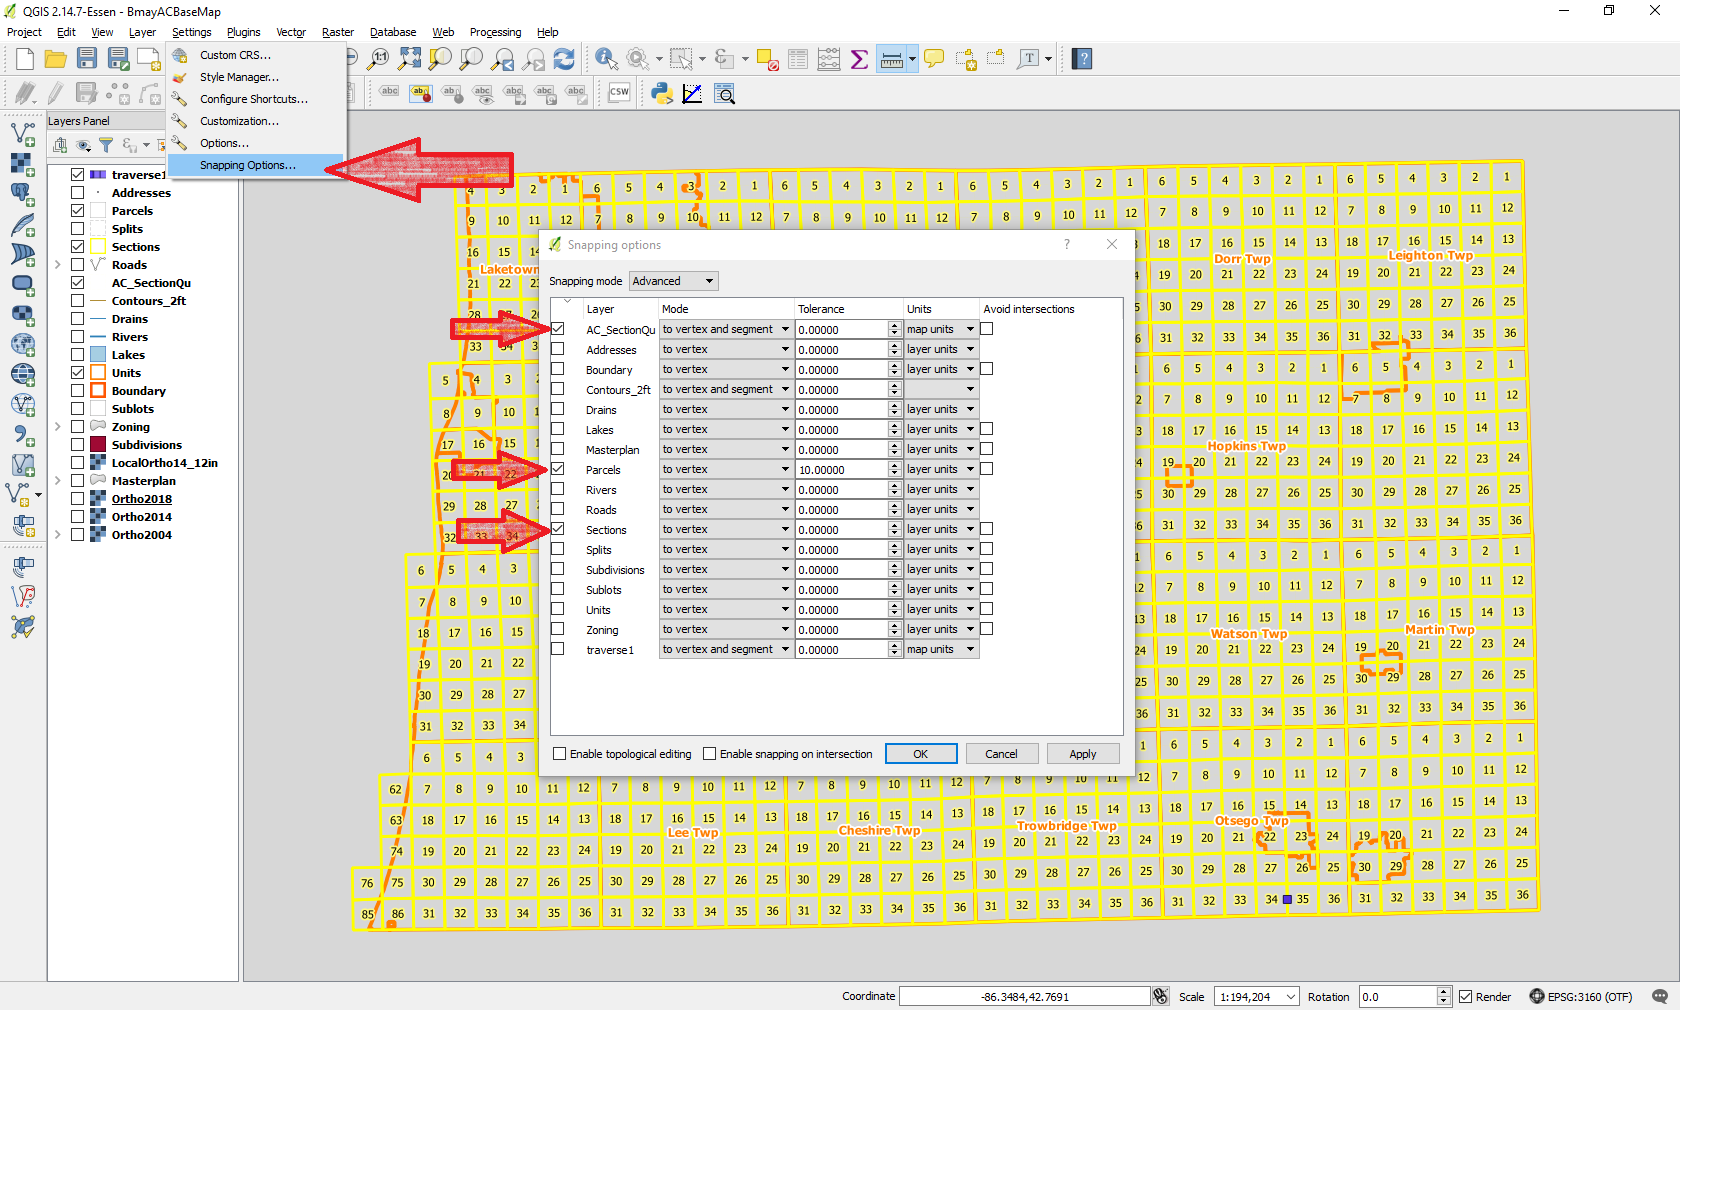
\includegraphics[scale=.20]{7.png}
\end{center}
\caption{Configure editing environment}
\end{figure}

\clearpage

\subsubsection{\Large Locate Point of Commencement}
To get to the Point of Commencement,
\medskip

Use \textbf{any combination} of the following methods:
\begin{itemize}
\item{Using Reference Layer}
\item{Using Measuring Tool}
\item{Search by Parcel Number \small(Search Layers Plugin)}
\item{Draw COGO lines \small(Azd Plugin)}\small(as described earlier)
\end{itemize}

\paragraph{Using Reference Layer}
\large Use reference layers; Units, AC\_SectionsQu, Sections, and Parcels.  Toggle layers on and off in Layers Panel and zoom in and out with mouse wheel.
\clearpage

\paragraph{Using Measuring Tool}
\large Use the measuring tool, make sure to set units to feet.  To exit current measurement right click (see fig.).
\begin{figure}[H]
\begin{center}
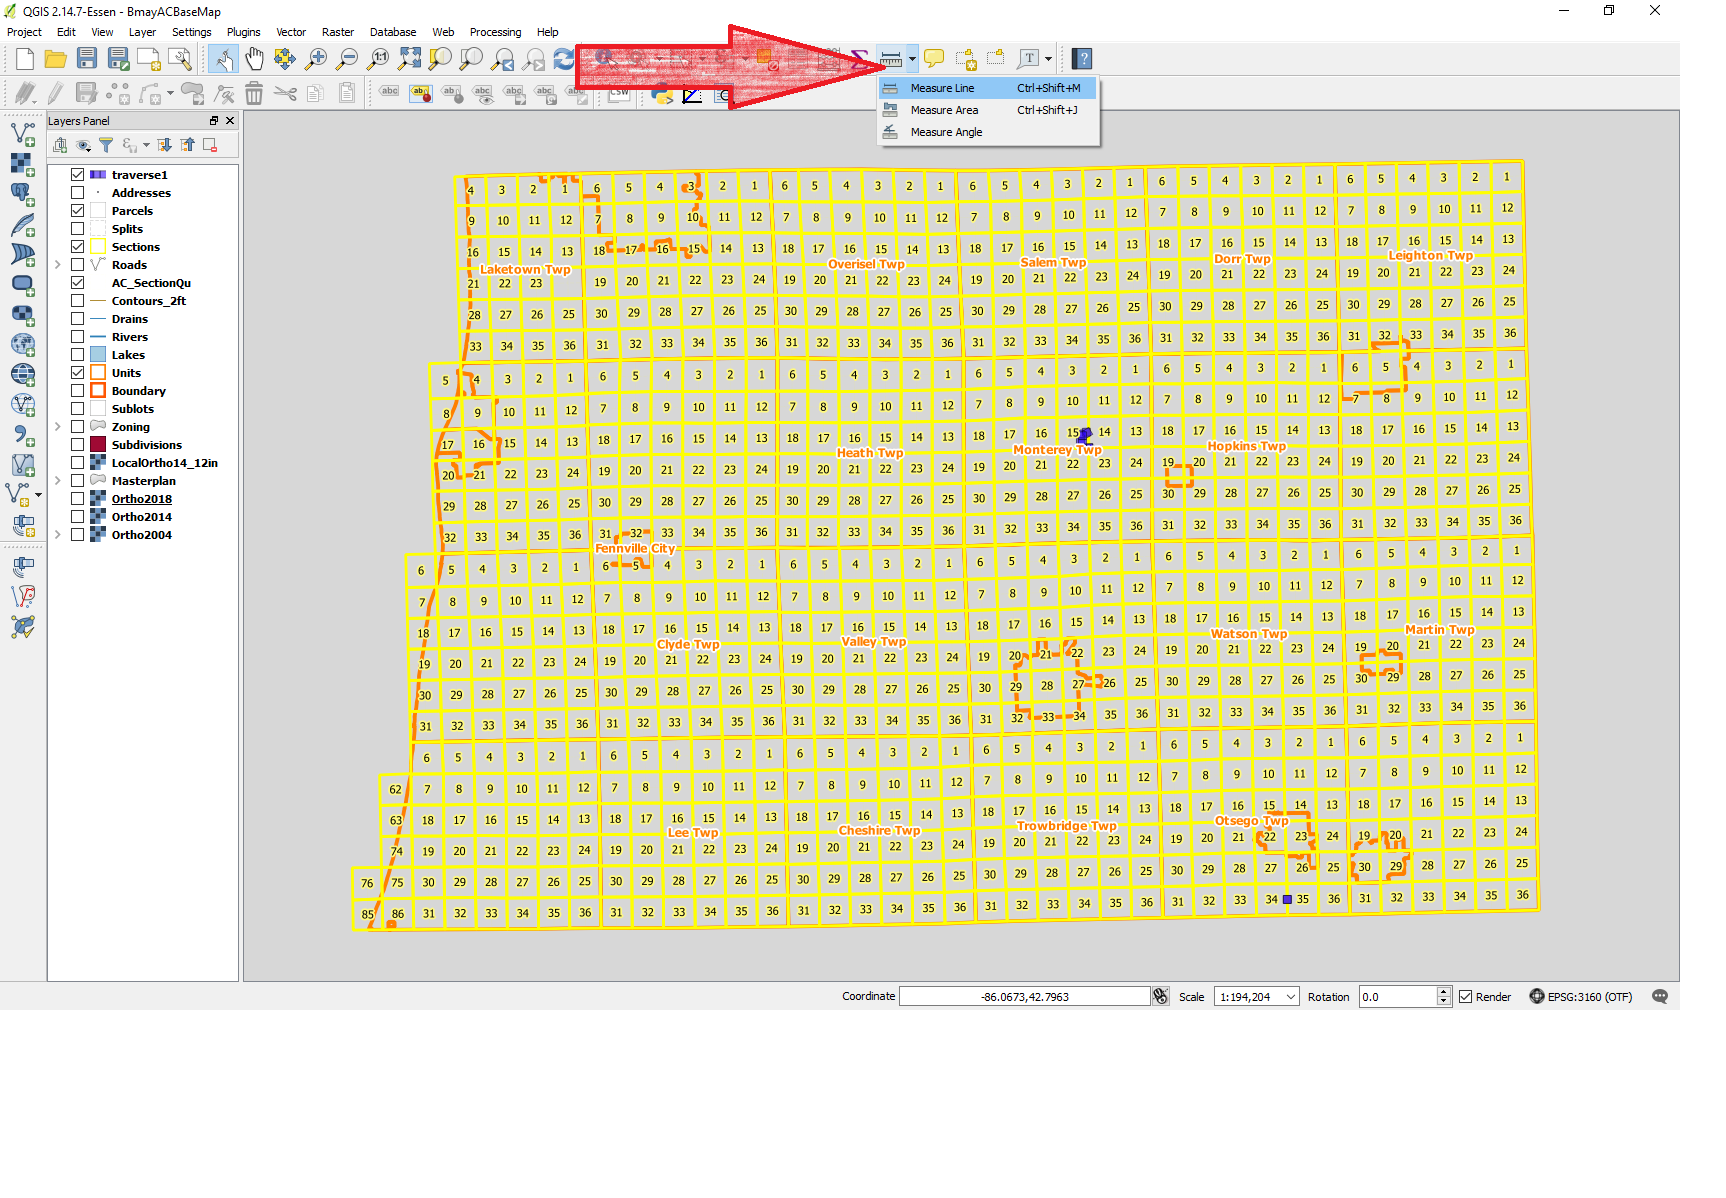
\includegraphics[scale=.20]{6.png}
\end{center}
\caption{Measuring Tool}
\end{figure}							
\clearpage
			
\paragraph{Search by Parcel Number}
\small (Search Layers Plugin.)
\subparagraph{}
To Launch Search Layers Plugin:\\In Plugins dropdown:\\Enable the \textbf{Search Layers} Plugin. (see fig.)		
\begin{figure}[H]
\begin{center}
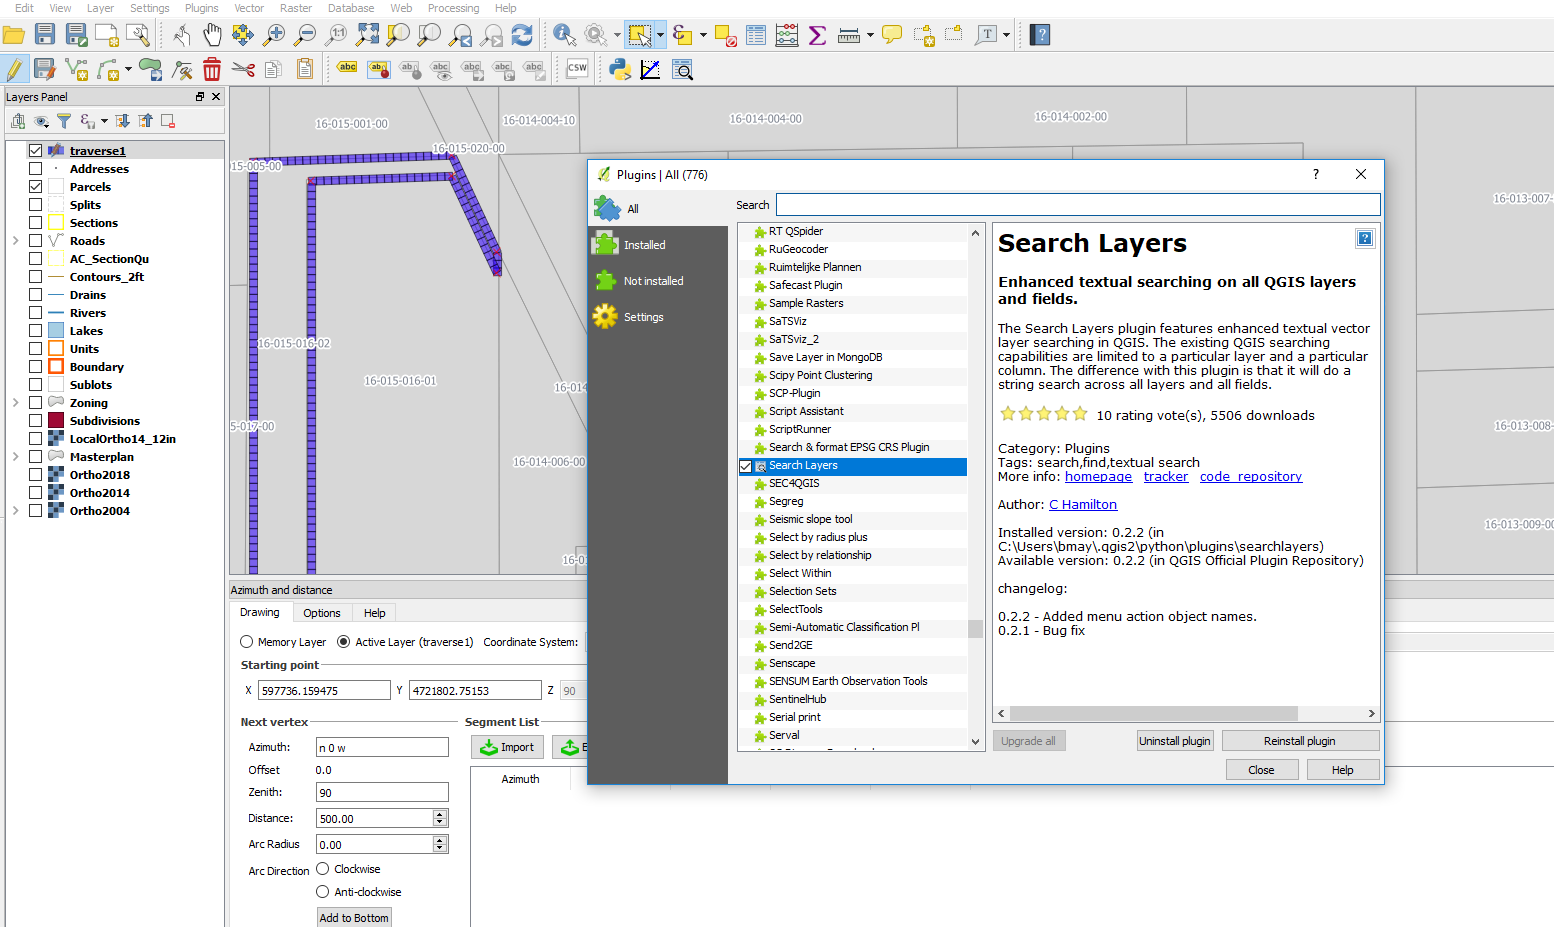
\includegraphics[scale=.20]{SearchLayers1b.PNG}
\end{center}
\caption{Search Layers Plugin}
\end{figure}
\bigskip
Enter parcel number {\tiny (with dashes)}, Set layers, and set search field.(see fig.) 
\begin{figure}[H]						
\begin{center}
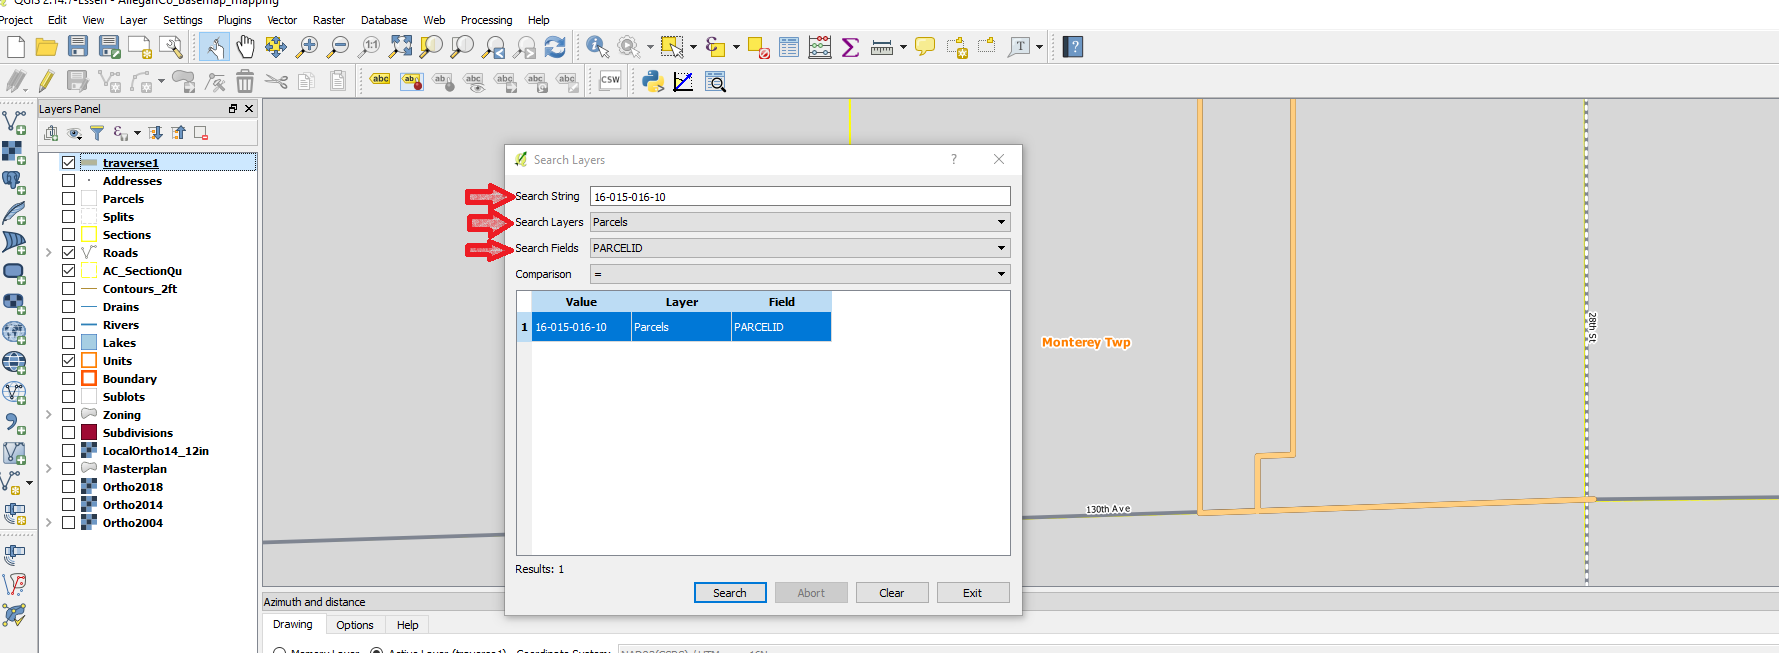
\includegraphics[scale=.20]{SearchLayers.png}
\end{center}
\caption{Search Layers Setup}
\end{figure}
											
\clearpage			
			
\end{document}
